\documentclass[12pt]{article} % use larger type; default would be 10pt

\usepackage{enumerate}
\usepackage{xeCJK}
\usepackage{mystyle}
\usepackage{ruby}
\usepackage{longtable}
\usepackage{hyperref}
\usepackage{amsthm,amssymb}
\usepackage[]{graphicx}

\theoremstyle{definition}
\newtheorem{question}{問}

\setCJKmainfont[AutoFakeBold=true]{Hiragino Mincho Pro} %my Mac
%\setCJKmainfont{MS PGothic} %AJP windows
%\renewcommand\rubysep{-5ex}
\newcommand{\kana}[2]{\ruby{#1}{#2}}
\newcommand{\mytabra}[1]{$\myabra{\mbox{#1}}$}

\title{2017年度S1数理科学基礎演習・微積分(理二三21−24)第3回}
\author{田中 雄一郎、Alex Leontiev、鈴木大}
\begin{document}
\maketitle
\begin{question}
	\begin{enumerate}[(1)]
		\item \begin{equation*}
				\begin{array}[]{c}
					f_x=y^2+2xy^3\\
					f_y=2xy+3x^2y^2
				\end{array}
			\end{equation*}
		\item \begin{equation*}
				\begin{array}[]{c}
					f_x=y\cos(xy)\\
					f_y=x\cos(xy).
				\end{array}
			\end{equation*}
	\end{enumerate}
\end{question}
\begin{question}
	\begin{enumerate}[(1)]
		\item \begin{equation*}
				\begin{array}[]{c}
					f_{xx}=2ax\\
					f_{xy}=f_{yx}=b\\
					f_{yy}=2c
				\end{array}
			\end{equation*}
		\item\begin{equation*}
				\begin{array}[]{c}
					f_{xx}=\left( 2a+4a^2x^2 \right)\exp\left( ax^2+by^2 \right)\\
					f_{xy}=f_{yx}= 4abxy\exp\left( ax^2+by^2 \right)\\
					f_{yy}=\left( 2b+4b^2y^2 \right)\exp\left(  ax^2+by^2\right).
				\end{array}
			\end{equation*}
	\end{enumerate}
\end{question}
\begin{question}
	\begin{enumerate}[(1)]
		\item 原点が最大になる(もちろん、極大にもなる):\begin{equation*}
				f(x,y)=-x^2+2xy-3y^2=-(x-y)^2-2y^2
			\end{equation*}
			になるので、yは0と等しくなかったら、$f(x,y)\le-2y^2<0=f(0,0)$になる。更に、$y$が0と等しくて、xは0でなかったら、
			$f(x,y)=-x^2<0$になる。
		\item 原点が極大にならない(もちろん、最大にもならない):\begin{equation*}
				f(x,y)=-x^2+3xy-2y^2=-\left( x-\frac{3}{2}y \right)^2+\frac{1}{4}y^2
			\end{equation*}
			になるので、$(x_n,y_n):=\left( \frac{3}{2n},\frac{1}{2n} \right)$ が原点に近づくが、$f(x_n,y_n)>0=f(0,0)$である。
			\begin{figure}[h!]
				\centering
				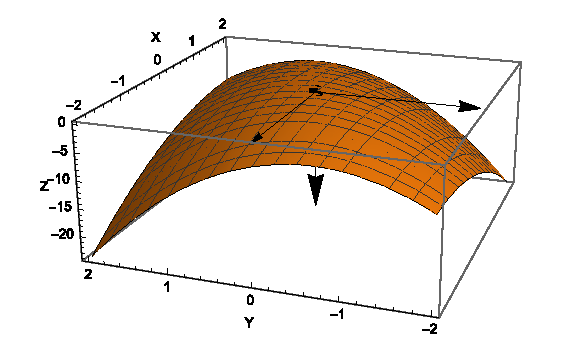
\includegraphics{3d1}
				\caption{問題3.(1)のグラフ}
			\end{figure}
	\end{enumerate}
\end{question}
\begin{question}
	\begin{enumerate}[(1)]
		\item 原点が極小にならない(もちろん、最小にもならない):
			$(x_n,y_n):=\left( -\frac{1}{n},0 \right)$ が原点に近づくが、$f(x_n,y_n)<0=f(0,0)$である。
		\item 原点が最小になる(もちろん、極小にもなる):
			yは0と等しくなかったら、$f(x,y)\ge y^4>0=f(0,0)$になる。更に、$y$が0と等しくて、xは0でなかったら、
			$f(x,y)=x^2>0$になっる。
			\begin{figure}[h!]
				\centering
				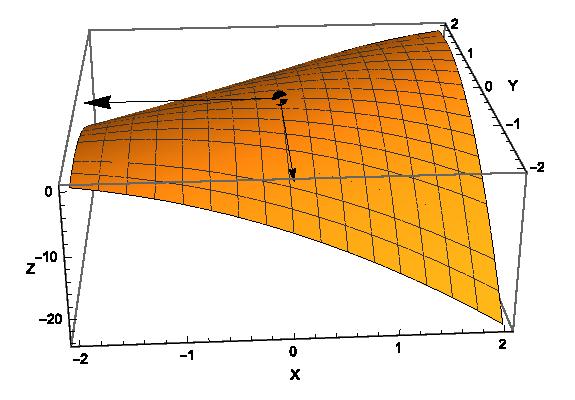
\includegraphics{3d2}
				\caption{問題3.(2)のグラフ}
			\end{figure}
	\end{enumerate}
\end{question}
\begin{question}
	\begin{enumerate}[(1)]
		\item 
			まず、勾配ベクトルを求めよ
			\begin{equation*}
				\begin{array}[]{c}
					f(x,y)=xy^2\\
					f_x(x,y)=y^2\\f_x(2,1)=1\\
					f_y(x,y)=2xy\\f_y(2,1)=4.
				\end{array}
			\end{equation*}
				なので、接平面が以下のようになる:\begin{equation*}
					\begin{array}[]{c}
						z-2=1\cdot(x-2)+4\cdot(y-1)\\
						x+4y-z=4.
					\end{array}
				\end{equation*}
			\begin{figure}[h!]
				\centering
				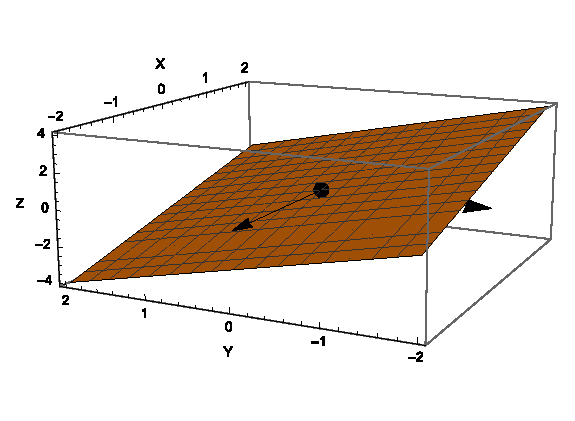
\includegraphics{4d1}
				\caption{問題4.(1)のグラフ}
			\end{figure}
		\item 
			まず、勾配ベクトルを求めよ
			\begin{equation*}
				\begin{array}[]{c}
					f(x,y)=2x^2-y^2\\
					f_x(x,y)=4x\\f_x(2,1)=8\\
					f_y(x,y)=-2y\\f_y(2,1)=-2.
				\end{array}
			\end{equation*}
				なので、接平面が以下のようになる:\begin{equation*}
					\begin{array}[]{c}
						z-7=8\cdot(x-2)-2\cdot(y-1)\\
						8x-2y-z=7.
					\end{array}
				\end{equation*}
			\begin{figure}[h!]
				\centering
				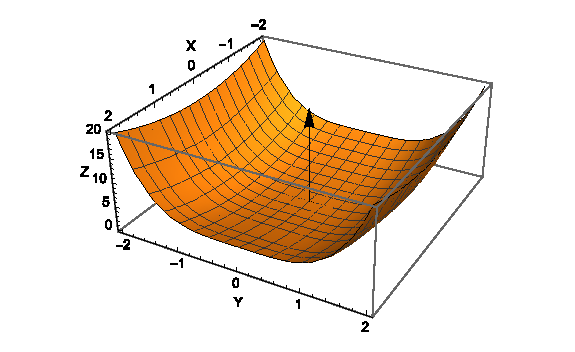
\includegraphics{4d2}
				\caption{問題4.(2)のグラフ}
			\end{figure}
	\end{enumerate}
\end{question}
\begin{question}
	\begin{enumerate}[(1)]
		\item まず、偏微分を求めよ:
			\begin{equation*}
				\begin{array}[]{c}
					f(x,y)=(x^2-y^2)^3\\
					f_x(x,y)=6x(x^2-y^2)^2\\
					f_y(x,y)=6y(x^2-y^2)^2.\\
				\end{array}
			\end{equation*}
			次、停留点を求めよ:\begin{equation*}
				\begin{array}[]{c}
					\left\{\begin{array}[]{l}
						6x(x^2-y^2)^2=0\\
						6y(x^2-y^2)^2=0\\
					\end{array}\right.\\[2em]
					\left\{\begin{array}[]{l}
						\left[\begin{array}[]{l}
							x=0\\
							x^2-y^2=0
						\end{array}\right.\\
						\left[\begin{array}[]{l}
							y=0\\
							x^2-y^2=0
						\end{array}\right.\\
					\end{array}\right.\\[2em]
					\left[\begin{array}[]{c}
						\left\{\begin{array}[]{l}
							x=0\\y=0
						\end{array}\right.\\
						x^2-y^2=0
					\end{array}\right.\\[2em]
					\left[
						\begin{array}[]{l}
x=y=0\\(x-y)(x+y)=0
						\end{array}
						\right.\\[2em]
						\left[\begin{array}[]{l}
							x=y=0\\x=y\\x=-y
						\end{array}\right.
				\end{array}
			\end{equation*}
			なので、停留点が:\begin{equation*}
				(0,0),\quad\left\{ (t,t)\mid t\in\R \right\},\quad \left\{ (t,-t)\mid t\in\R \right\}.
			\end{equation*}
		\item まず、偏微分を求めよ:
			\begin{equation*}
				\begin{array}[]{c}
					f(x,y)=(x^2+y^2)\exp\left(-x^2-y^2  \right)\\
					f_x(x,y)=2x(1-x^2-y^2)\exp\left( -x^2-y^2 \right)\\
					f_x(x,y)=2y(1-x^2-y^2)\exp\left( -x^2-y^2 \right).\\
				\end{array}
			\end{equation*}
			次、停留点を求めよ:\begin{equation*}
				\begin{array}[]{c}
					\left\{\begin{array}[]{l}
					2x(1-x^2-y^2)\exp\left( -x^2-y^2 \right)=0\\
					2y(1-x^2-y^2)\exp\left( -x^2-y^2 \right)=0\\
					\end{array}\right.\\[2em]
					\left\{\begin{array}[]{l}
						\left[\begin{array}[]{l}
							x=0\\
							1-x^2-y^2=0
						\end{array}\right.\\
						\left[\begin{array}[]{l}
							y=0\\
							1-x^2-y^2=0
						\end{array}\right.\\
					\end{array}\right.\\[2em]
					\left[\begin{array}[]{c}
						\left\{\begin{array}[]{l}
							x=0\\y=0
						\end{array}\right.\\
						x^2+y^2=1.
					\end{array}\right.
				\end{array}
			\end{equation*}
			なので、停留点が:\begin{equation*}
				(0,0),\quad\left\{ (\cos(t),\sin(t))\mid 0\le t<2\pi \right\}.
			\end{equation*}
	\end{enumerate}
\end{question}
\begin{question}
	$(x_n,y_n):=\left( 1/n,1/n \right)$とする。そうしたら、\begin{equation*}
		\begin{array}[]{c}
			(x_n,y_n)\to(0,0)\\
			f(x_n,y_n)
			=1/2.
		\end{array}
	\end{equation*}
		なので、$(x_n,y_n)$が原点に収束するが、$f(x_n,y_n)$が$f(0,0)=0$に収束しない。
\end{question}
\begin{question}
	\begin{equation*}
		\begin{array}[]{c}
			f_x(x,y)=\left\{\begin{array}[]{ll}
				\frac{\partial}{\partial x}\left( xy\frac{x^2-y^2}{x^2+y^2} \right)&(x,y)\neq(0,0)\\
				\lim_{h\to0}\frac{f(h,0)}{h}&(x,y)=(0,0)
			\end{array}\right.\\
			=\left\{\begin{array}[]{ll}
				\frac{x^4y-y^5-4x^2y^3}{\left( x^2+y^2 \right)^2}&(x,y)\neq(0,0)\\
				\lim_{h\to0}\frac{0}{h}=0&(x,y)=(0,0)
			\end{array}\right.\\
			f_y(x,y)=\left\{\begin{array}[]{ll}
				\frac{\partial}{\partial y}\left( xy\frac{x^2-y^2}{x^2+y^2} \right)&(x,y)\neq(0,0)\\
				\lim_{h\to0}\frac{f(0,h)}{h}&(x,y)=(0,0)
			\end{array}\right.\\
			=\left\{\begin{array}[]{ll}
				\frac{x^5-xy^4-4x^3y^2}{\left( x^2+y^2 \right)^2}&(x,y)\neq(0,0)\\
				\lim_{h\to0}\frac{0}{h}=0&(x,y)=(0,0)
			\end{array}\right.\\
			f_{xy}(0,0)=\lim_{h\to0}\frac{f_x(0,h)}{h}=\lim_{h\to0}\frac{-h^5}{h^5}=-1\\
			f_{yx}(0,0)=\lim_{h\to0}\frac{f_y(h,0)}{h}=\lim_{h\to0}\frac{h^5}{h^5}=1\\
%%			=\left\{\begin{array}[]{ll}
%%				\frac{x^4y-y^5-4x^2y^3}{\left( x^2+y^2 \right)^2}&(x,y)\neq(0,0)\\
%%				\lim_{h\to0}\frac{0}{h}=0&(x,y)=(0,0)
%%			\end{array}\right.\\
			\mbox{なので、$f_{xy}\neq f_{yx}$}
		\end{array}
	\end{equation*}
\end{question}
\begin{question}
	まず、$f_x$を求めよ:\begin{equation*}
		\begin{array}[]{c}
			f_x(x,y)=\left\{\begin{array}[]{ll}
				\frac{\partial}{\partial x}\left( xy\sin\frac{1}{\sqrt{x^2+y^2}} \right)&(x,y)\neq(0,0)\\
				\lim_{h\to0}\frac{f(h,0)}{h}&(x,y)=(0,0)
			\end{array}\right.\\
			=\left\{\begin{array}[]{ll}
				y\sin\frac{1}{\sqrt{x^2+y^2}}-x^2y\left( x^2+y^2 \right)^{-\frac{3}{2}}\cos\frac{1}{\sqrt{x^2+y^2}}&(x,y)\neq(0,0)\\
				\lim_{h\to0}\frac{0}{h}=0&(x,y)=(0,0)
			\end{array}\right.
		\end{array}
	\end{equation*}
		以下なように$(x_n,y_n)$をとる:
		\begin{equation*}
			(x_n,y_n):=\left( a_n,a_n \right),\quad a_n:=\frac{1}{2\sqrt{2}\pi n}
		\end{equation*}
		そうすると$(x_n,y_n)\to0$が、
		\begin{equation*}
			\begin{array}[]{c}
				\lim_{n\to\infty}f_x(x_n,y_n)=
				\underbrace{\lim_{n\to\infty}y_n\sin\frac{1}{\sqrt{x_n^2+y_n^2}}}_{\myabs{y_n\sin\frac{1}{\sqrt{x_n^2+y_n^2}}}\le\myabs{y_n}\to0}
				-\lim_{n\to\infty}x_n^2y_n\left( x_n^2+y_n^2 \right)^{-\frac{3}{2}}
				\cos\frac{1}{\sqrt{x_n^2+y_n^2}}\\
				=\lim_{n\to\infty}\frac{a_n^3}{2\sqrt{2}a_n^3}\cos\frac{1}{\sqrt{2}a_n}=\frac{1}{2\sqrt{2}}\cos\left( 2\pi n \right)=\frac{1}{2\sqrt{2}}\neq0.
			\end{array}
		\end{equation*}
		なので、$f_x$が原点で連続ではない。
\end{question}
\begin{question}
	原点を通る線
	\begin{equation*}
		ax+by=0,\quad a^2+b^2>0
	\end{equation*}
	を一個とる。
	この線のそれぞれの点が以下のように表せる:
	\begin{equation*}
		(-bt,at),\quad t\in\R.
	\end{equation*}
	そうすると、その微分が
	\begin{equation*}
		\begin{array}[]{c}
			\lim_{t\to0}\frac{f(-bt,at)}{\mynorm{(-bt,at)}}=\lim_{t\to0}\frac{-abt^2}{(b^2t^2+at)t\sqrt{a^2+b^2}}=-\frac{ab}{a\sqrt{a^2+b^2}}.
		\end{array}
	\end{equation*}
\end{question}
\end{document}




